\documentclass[11pt]{article}

\usepackage[margin=1in]{geometry}
\usepackage{amsmath,amssymb,mathtools}
\usepackage{graphicx}
\usepackage{xcolor}
\usepackage{hyperref}
\usepackage{enumitem}

\hypersetup{colorlinks=true,linkcolor=blue,citecolor=blue,urlcolor=blue}
\setlength{\parindent}{0pt}
\setlength{\parskip}{0.65em}
\newcommand{\dd}{\mathrm d}
\newcommand{\Tr}{\operatorname{Tr}}
\newcommand{\T}{\mathcal T}

\title{Functional Renormalization Group Notes\\\large }
\author{P. Shubham Parashar}
\date{June 2024}

\begin{document}
\maketitle

\begin{abstract}
These notes collect two related pieces of functional-renormalization-group machinery: the standard fermionic fRG setup with a cutoff-dependent quadratic kernel, single-scale propagator, and Katanin substitution; and the spin fRG construction for an anisotropic Heisenberg model, including deformation of longitudinal/transverse couplings, hybrid functionals, spontaneous symmetry breaking, and the vertex hierarchy. This is a working note. Signs, regulator conventions, factors of $\beta N$, and the exact meaning of the Katanin replacement should be checked.
\end{abstract}

\section{Fermionic fRG: minimal setup}

Start from a Grassmann functional integral
\begin{equation}
\mathcal Z=\int \mathcal D(\bar\psi,\psi)\,e^{-S(\bar\psi,\psi)}.
\end{equation}
Separate the quadratic and interacting parts as
\begin{equation}
S(\bar\psi,\psi)=(\bar\psi,Q\psi)-\widetilde V(\bar\psi,\psi),
\qquad
(\bar\psi,Q\psi)=\sum_j\bar\psi_jQ_j\psi_j.
\end{equation}
For a translationally invariant fermion problem the composite index is typically $j=(i\omega_n,\mathbf k,s)$ and
\begin{equation}
Q_j=i\omega_n-\xi_{\mathbf k},\qquad \xi_{\mathbf k}=\varepsilon_{\mathbf k}-\mu.
\end{equation}
The inverse of the quadratic kernel is the bare propagator, $G_0=Q^{-1}$, up to sign and normalization conventions.

\section{Cutoff and single-scale propagator}

Introduce a cutoff-dependent quadratic kernel
\begin{equation}
Q^\Lambda=Q/\chi(\Lambda),
\qquad
\chi(\Lambda)\approx \Theta(|\xi|-\Lambda).
\end{equation}
The flow starts near a bandwidth scale $\Lambda_i\sim W$ and ends at $\Lambda_f=0$, where $\chi(0)=1$. The full propagator is
\begin{equation}
G^\Lambda=\left(Q^\Lambda-\Sigma^\Lambda\right)^{-1}.
\end{equation}
The single-scale propagator is the derivative of $G^\Lambda$ at fixed self-energy:
\begin{equation}
S^\Lambda=-G^\Lambda\dot Q^\Lambda G^\Lambda,
\qquad \dot Q^\Lambda=\partial_\Lambda Q^\Lambda.
\end{equation}
For a sharp-shell cutoff, $\dot\chi$ produces a delta function on the running shell $|\xi_{\mathbf k}|=\Lambda$.

\begin{figure}[h]
\centering
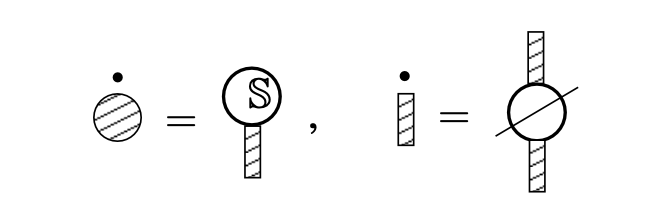
\includegraphics[width=0.75\linewidth]{../../assets/images/notes/functional-rg/flow2.png}
\caption{Schematic self-energy and two-particle vertex flow. The vertex flow uses the Katanin modification.}
\end{figure}

\section{Katanin replacement}

At the usual one-loop truncation level, the self-energy and two-particle vertex obey closed flow equations after higher vertices are either neglected or approximated. Diagrammatically, the self-energy flow contains one single-scale line and one two-particle vertex, while the two-particle vertex flow contains particle-particle and particle-hole loop corrections.

The Katanin replacement promotes the single-scale structure in the two-particle flow according to
\begin{equation}
S^\Lambda G^\Lambda+G^\Lambda S^\Lambda
\longrightarrow
\partial_\Lambda\left(G^\Lambda G^\Lambda\right).
\end{equation}
Equivalently, this accounts for the self-energy feedback term contained in $\partial_\Lambda G^\Lambda$ inside the corresponding two-particle loop.

\textbf{Convention warning.} Do not globally replace every $S^\Lambda$ by $\partial_\Lambda G^\Lambda$ without checking the truncation. The Katanin substitution is a controlled modification of the two-particle flow.

\section{Summation trick}

Momentum sums can often be reduced to energy integrals,
\begin{equation}
\sum_{\mathbf k}\longrightarrow \int_{-W}^{W}\dd\varepsilon\,\rho(\varepsilon).
\end{equation}
If the scale dependence enters only through $\chi$ and $\Sigma$, then for an integrand $\mathcal I(\xi,\chi,\Sigma)$,
\begin{equation}
\int_{-W}^{W}\dd\varepsilon\,\rho(\varepsilon)\,\partial_\Lambda\mathcal I
=\int_{-W}^{W}\dd\varepsilon\,\rho(\varepsilon)
\left(
\dot\chi\frac{\partial\mathcal I}{\partial\chi}
+\dot\Sigma\frac{\partial\mathcal I}{\partial\Sigma}
\right).
\end{equation}
For a sharp cutoff this becomes
\begin{equation}
\int\dd\varepsilon\,\rho(\varepsilon)
\left[
\left.\mathcal I\right|_{\chi=1}\delta(|\varepsilon|-\Lambda)
+\dot\Sigma\frac{\partial\mathcal I}{\partial\Sigma}
\right].
\end{equation}

\section{Spin fRG deformation scheme}

For the anisotropic Heisenberg model, write
\begin{equation}
\mathcal H=\mathcal H_0+\mathcal V,
\end{equation}
with
\begin{equation}
\mathcal V=-\frac12\sum_{ij}
\left[J_{ij}^{\perp}\left(S_i^+S_j^-+S_i^-S_j^+\right)+J_{ij}^{z}S_i^zS_j^z\right].
\end{equation}
The deformation parameter $\Lambda$ is introduced through
\begin{equation}
J_{\Lambda,ij}^{\perp}=J_{ij}^{\perp}-R_{\Lambda,ij}^{\perp},
\qquad
J_{\Lambda,ij}^{z}=J_{ij}^{z}-R_{\Lambda,ij}^{z}.
\end{equation}
The regulator is chosen so that the initial point is solvable and the final point recovers the physical model.

\begin{figure}[h]
\centering
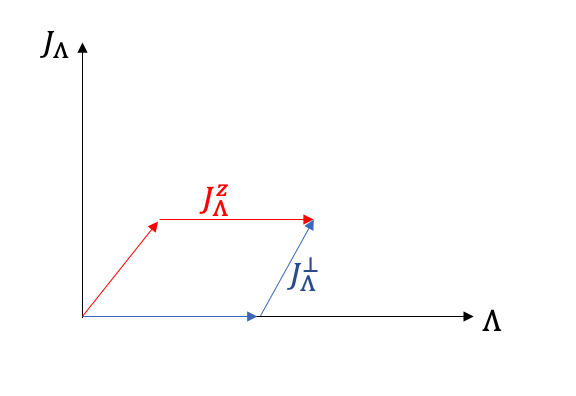
\includegraphics[width=0.58\linewidth]{../../assets/images/notes/functional-rg/deformation.png}
\caption{Example deformation: longitudinal fluctuations are switched on first, followed by transverse fluctuations.}
\end{figure}

\section{Generating functional and exact flow}

Define the connected generating functional
\begin{equation}
\mathcal G_\Lambda[\mathbf h]
=\ln\Tr\left[e^{-\beta\mathcal H_0}
\mathcal T\exp\left\{\int_0^\beta\dd\tau
\left[\sum_i\mathbf h_i(\tau)\cdot\mathbf S_i(\tau)-\mathcal V_\Lambda(\tau)\right]
\right\}\right].
\end{equation}
Connected spin correlators are
\begin{equation}
G_{\Lambda,I_1\cdots I_n}^{\alpha_1\cdots\alpha_n}
=\left.
\frac{\delta^n\mathcal G_\Lambda[\mathbf h]}
{\delta h_{I_1}^{\bar\alpha_1}\cdots\delta h_{I_n}^{\bar\alpha_n}}
\right|_{h=0}.
\end{equation}
After a modified Legendre transform, the irreducible functional obeys
\begin{equation}
\partial_\Lambda\mathcal L_\Lambda[\mathbf M]
=\frac12\Tr\left[
\left(\mathcal L_\Lambda''[\mathbf M]+\mathcal R_\Lambda\right)^{-1}
\partial_\Lambda\mathcal R_\Lambda
\right].
\end{equation}

\section{Hybrid functional and longitudinal amputation}

A Hubbard-Stratonovich decoupling of the longitudinal sector motivates a hybrid functional
\begin{equation}
\mathcal F_\Lambda[\mathbf h^\perp,s]
=\mathcal G_\Lambda\left[\mathbf h^\perp,
 h_i^z=\sum_jJ_{\Lambda,ij}^zs_j\right]
+\frac12\sum_{IJ}\mathbb J^z_{\Lambda,IJ}s_Is_J.
\end{equation}
Its derivatives define objects connected in the transverse sector and amputated in the longitudinal sector. For example,
\begin{align}
F_{\Lambda,I}^{z}&=\sum_J\mathbb J^z_{\Lambda,IJ}G_{\Lambda,J}^{z},\\
F_{\Lambda,IJ}^{zz}
&=\sum_{KL}\mathbb J^z_{\Lambda,IK}\mathbb J^z_{\Lambda,JL}G_{\Lambda,KL}^{zz}
+\mathbb J^z_{\Lambda,IJ}.
\end{align}

\section{Symmetry-broken phase}

In the ordered phase,
\begin{equation}
\langle S_I^\alpha\rangle_\Lambda=M_\Lambda\delta^{\alpha z}.
\end{equation}
In the hybrid representation the corresponding longitudinal exchange field is
\begin{equation}
\bar\Phi_{I,\Lambda}^\alpha=\phi_\Lambda\delta^{\alpha z},
\qquad
\phi_\Lambda=J^z_{\Lambda,0}M_\Lambda.
\end{equation}

\section{Tree-level two-point identities}

In momentum-frequency space, $K=(\mathbf k,i\omega)$,
\begin{align}
F_\Lambda^{+-}(K)&=\left[\Gamma_\Lambda^{+-}(K)+R_{\Lambda,k}^{\perp}\right]^{-1},\\
F_\Lambda^{zz}(K)&=\left[\Gamma_\Lambda^{zz}(K)+R_{\Lambda,k}^{\phi}\right]^{-1}.
\end{align}
The transverse connected and partially amputated functions coincide,
\begin{equation}
G_\Lambda(K)=G_\Lambda^{+-}(K)=F_\Lambda^{+-}(K),
\end{equation}
whereas the longitudinal relation is
\begin{equation}
F_\Lambda(K)=F_\Lambda^{zz}(K)=\left(J^z_{\Lambda,k}\right)^2G_\Lambda^{zz}(K)+J^z_{\Lambda,k}.
\end{equation}
Thus,
\begin{align}
\Gamma_\Lambda^{+-}(K)&=G_\Lambda^{-1}(K)+J_{\Lambda,k}^{\perp}-J_k^{\perp},\\
\Gamma_\Lambda^{zz}(K)
&=-\frac{G_\Lambda^{zz}(K)}{1+J^z_{\Lambda,k}G_\Lambda^{zz}(K)}+\frac{1}{J_k^z}.
\end{align}

\section{Vertex-flow hierarchy}

Expanding the exact functional flow produces an infinite hierarchy of coupled integro-differential equations for the vertices $\Gamma_{\Lambda,K_1\cdots K_n}^{\alpha_1\cdots\alpha_n}$.

\begin{figure}[h]
\centering
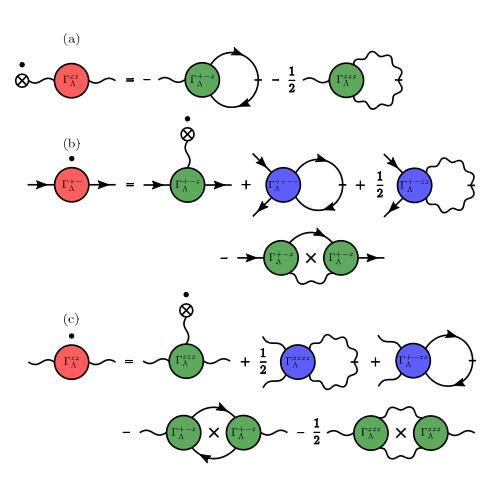
\includegraphics[width=0.58\linewidth]{../../assets/images/notes/functional-rg/vertex-flow.png}
\caption{Representative vertex-flow hierarchy diagram from the original notes.}
\end{figure}

The free-energy flow is schematically
\begin{equation}
\partial_\Lambda f_\Lambda
=\int_KG_\Lambda(K)\partial_\Lambda R^\perp_{\Lambda,k}
+\frac12\int_K\left[F_\Lambda(K)-J^z_{\Lambda,k}\right]\partial_\Lambda R^\phi_{\Lambda,k}
-\frac12\phi_\Lambda^2\partial_\Lambda R^\phi_{\Lambda,0}.
\end{equation}
The exchange-field flow is fixed by removing the linear fluctuation term:
\begin{equation}
\Gamma_\Lambda^{zz}(0)\partial_\Lambda\phi_\Lambda
=-\partial_\Lambda\left(R^\phi_{\Lambda,0}\phi_\Lambda\right)
-\int_K\dot G_\Lambda(K)\Gamma_\Lambda^{+-z}(K,-K,0)
-\frac12\int_K\dot F_\Lambda(K)\Gamma_\Lambda^{zzz}(K,-K,0).
\end{equation}
The transverse and longitudinal single-scale propagators are
\begin{equation}
\dot G_\Lambda(K)=-G_\Lambda^2(K)\partial_\Lambda R^\perp_{\Lambda,k},
\qquad
\dot F_\Lambda(K)=-F_\Lambda^2(K)\partial_\Lambda R^\phi_{\Lambda,k}.
\end{equation}

\section{Infinite-range / Katanin benchmark}

The original note attempted a benchmark in an infinite-range limit, comparing a Katanin-corrected flow with a tree-level vertex-corrected flow. The running gap was
\begin{equation}
\Delta_\Lambda=H\frac{M_0}{M_\Lambda},
\end{equation}
and the magnetization flow had the schematic form
\begin{equation}
\partial_\Lambda M_\Lambda
=\frac{M_0}{\beta N}\sum_{\mathbf k,\omega}
\frac{\Gamma^{+-z}_{\Lambda,\mathrm{Kat}}\delta(k-\Lambda)}
{\Delta_\Lambda+E_{\mathbf k}-i\omega}.
\end{equation}

\begin{figure}[h]
\centering
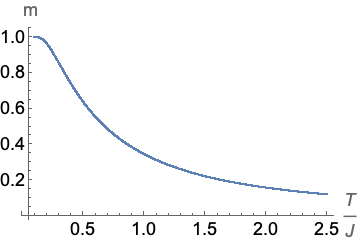
\includegraphics[width=0.43\linewidth]{../../assets/images/notes/functional-rg/katanin-0.01.png}\hfill
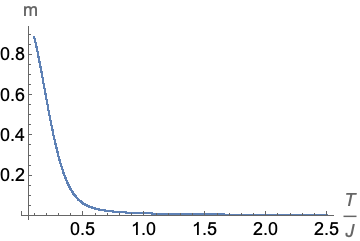
\includegraphics[width=0.43\linewidth]{../../assets/images/notes/functional-rg/vertex-0.001.png}
\caption{Original diagnostic plots: Katanin correction and vertex correction.}
\end{figure}

\textbf{Audit warning.} This benchmark is the least polished part of the note. The susceptibility scaling and the $H\to0$ limit should be rederived before reuse.

\section{Next steps}

\begin{enumerate}[leftmargin=*]
\item Decide whether the active target is fermionic fRG, spin fRG, or only the Katanin benchmark.
\item Fix the regulator convention and state it once in a boxed definition.
\item Redo the infinite-range benchmark independently in a two-page derivation.
\item Only then decide whether this connects to the quantum-Hall spin-splitting project.
\end{enumerate}

\begin{thebibliography}{9}
\bibitem{SalmhoferHonerkamp2001}
M. Salmhofer and C. Honerkamp, ``Fermionic renormalization group flows,'' Prog. Theor. Phys. \textbf{105}, 1 (2001).

\bibitem{Katanin2004}
A. A. Katanin, ``Fulfillment of Ward identities in the functional renormalization group approach,'' Phys. Rev. B \textbf{70}, 115109 (2004).

\bibitem{GerschHonerkampRoheMetzner2005}
R. Gersch, C. Honerkamp, D. Rohe, and W. Metzner, ``Fermionic renormalization group flow into phases with broken discrete symmetry: charge-density wave mean-field model,'' Eur. Phys. J. B \textbf{48}, 349 (2005).
\end{thebibliography}

\end{document}
